\documentclass[aps,prb,groupedaddress,twocolumn]{revtex4}
\usepackage{amsmath}
\usepackage{color}
\usepackage{graphicx}
\usepackage{verbatim}
\usepackage{graphicx}

\usepackage[normalem]{ulem}	% Part of the standard distribution
\bibliographystyle{apsrev}


\newcommand{\note}[1]{
{\color{red} \bf{#1}}}

\begin{document}

\title{Designer Hamiltonians---bridging lattice-scale physics \\ and continuum field theory with 
quantum Monte Carlo simulations} 

\author{Ribhu K. Kaul}
\email[]{rkka@pa.uky.edu}
\affiliation{Department of Physics and Astronomy, University of
  Kentucky, Lexington, Kentucky 40506, USA}
\author{Roger G. Melko}
\email[]{rgmelko@uwaterloo.ca}
\affiliation{Department of Physics and Astronomy, University of Waterloo, Ontario, N2L 3G1, Canada}
\author{Anders W. Sandvik}
\email[]{sandvik@bu.edu}
\affiliation{Department of Physics, Boston University, 590 Commonwealth Avenue, Boston, Massachusetts 02215, USA}


\date{\today}

\begin{abstract}
We discuss recent large-scale numerical studies of ``designer Hamiltonians'', which are lattice models tailored 
specifically to be free from sign problems when simulated with quantum Monte Carlo methods but still can host 
complex  many-body states and quantum phase transitions of great interest in condensed matter physics and quantum 
information theory. We here focus on quantum spin systems in which competing interactions lead to non-magnetic 
ground states. These states and their associated quantum phase transitions can be studied in great detail
and allow direct connections with universal properties of low-energy effective quantum field theories. As 
specific examples, we discuss the transition from a N\'eel antiferromagnet to either a featureless quantum 
paramagnet or a valence-bond-solid (VBS) in SU($2$) and SU($N$) spin models, as well as spin liquid and an
associated XY$^*$ transition in XXZ systems. We also discuss recent progress on quantum Monte Carlo algorithms, 
including ground state projection in the valence-bond basis and direct computation of the Renyi variants of 
the entanglement entropy.
\end{abstract}


\pacs{}

%\keywords{}

\maketitle

\section{Introduction}

Quantum field theory has emerged as one of the most fruitful approaches for studying low-energy properties of
complex strongly correlated and entangled quantum matter systems. There are potential pitfalls and difficulties 
with this approach, however, and it is important to also study systems directly based on the Hamiltonian 
formulation. One of the most fruitful directions is to use numerical methods to study lattice hamiltonians 
in an unbiased way, and to extract from such calculations the relevant low-energy emergent properties that can 
be compared with results for corresponding quantum field theories. Such connections 
between the two approaches can have significant synergy effects in advancing our understanding of many-body 
phenomena. Computational studies have their own challenges, however, and most systems of interest are currently 
beyond the reach of existing numerical algorithms. Frustrated quantum spin systems and fermions in two and three 
dimensions are the two main groups of problematic systems. The approach we review here is to tailor particular 
``designer hamiltonians'', which can host ground states and quantum phase transitions of interest and also are 
amenable to large-scale numerical studies. The computational technique we have in mind is quantum Monte Carlo 
(QMC) simulatuons, which in the aforementioned systems are normally affected by the infamous ``sign problem'', 
i.e., the weight function in the configuration space constructed using the path integral or other mappings to 
an effective statistical-mechanics problem is not positive definite (and hence cannot be directly used as 
a probability distribution for importance sampling).

According to one interpretation of Murphy's law, interesting designer Hamiltonians should not exist---if a 
model is sign-problem free, it must be trivial or uninteresting. There are already many counter examples to this
pessimistic view, however, and we will here review some recent examples in the area of quantum magnetism. 
Moreover, recent advances in QMC methods have made it possible to truly approach the low-energy limit of
such models and to make detailed connections with field theories. We will brifly address some of these technical 
advances as well. First, let us discuss the drawbacks of field theory and the philosophy of the synergistic
use of designer hamiltonians  in some more detail.

A field theory can rarely be rigorously derived exactly from 
an underlying Hamiltonian (which is the natural starting point for describing condensed matter systems). Instead
it is constructed based on symmetries, in combination with insights or assumptions on the physical nature of the
system. Some times the field theory can be derived in some well defined limit, e.g., the $(D+1)$-dimensional
nonlinear $\sigma$ model description of interacting quantum spins in $D$ dimensions was derived by Haldane in 
the semi-classical limit of large spin $S$ by using coherent spin states. Having identified or proposed a field
theory, the next step is to extract its properties. Often this is done using the renormalization group (RG)
approach, which may result in flows to some previously known fixed point, or to some fixed point or effective
model whose properties are not known. The RG itsef may have to rely on approximations that are not always easy
to justify, and if the flow is to some unknown state, it may be challenging to characterize it. Often the theory
is modified in such a way that it can be rigoroulsy controlled and the physical situation of interest is studied 
by some expansion around it. Well known examples are the $\epsilon$ expansion around the upper critical dimension 
and the $1/N$ expansion in the number of components $N$ (spin components, flavors of fermions, etc). The
extrapolation to the $\epsilon$ or $N$ of main interest is often difficult.

Because of issues such as these, it is important to test the predictions of field theories in some way. In some
cases there are exact solutions, e.g., the Bethe Ansatz solution of the $S=1/2$ Heisenberg chain has been immensely
important for testing the non-linear sigma model description of this class of critical spin chains. The exact
AKLT state for a special version of the $S=1$ chain was similarly important in testing Haldane's prediction of
the qualitative differences between half-odd integer and integer spins. Exact solutions are rare, however, and
essentially limited to one dimensional. Another, more general approach is to study Hamiltonians numerically. Exact
diagonalization of the Hamiltonian is possible only for small systems, which limits the usefulness of this approach 
to some one dimensional systems. White's density matrix renormalization (DMRG) scheme and related approaches based 
on matric-product states have enabled even more detailed studies of the low-energy physics of 1D systems (including
also ``ladders'' of several coupled chains). While there has been some progress for two-dimensional systems, with
DMRG and tensor-product states (generalizations of matrix-product states), in general these approaches have not
yet reached the level where one can obtain unbiased results for large systems.

The only numerical approach with which one can reach sufficiently large lattices in two and three dimensions
is QMC simulations, and, as already noted, they are often limited in practice by sign problems. The class of
models for there is no sign problem, or it is known how to circumvent it, still contains a vast range of 
models with non-trivial and interesting ground states and quantum phase transitions.

...Microscopic interactions do not have to correspond to any particular 
material, the idea is to tailor a system in such a way that it contains a particular macroscopic (low-energy) 
phenomenon of interest - universal physics is captured. We will call such models ``Designer Hamiltonians''.
With unbiased large-scale simulations of Designer Hamiltonians one can test field theories proposed to 
capture specific quantum many-body states or quantum phase transitions. Explorations of Designer Hamiltonians
can also serve as ``experiments'' for discovering novel phenomena (examples...?).


Mention that impurities and disorder is interesting but will not be discussed here.

\section{Modern QMC methods}




\subsection{Finite-T and T=0 projector methods presented in a common
  framework}
\label{ss:method}

Mention determinant-based fermion QMC (without details)

\subsection {Generalizations from SU(2) to SU(N)}
\label{ss:su2N}

Both methods discussed in the previous section can be generalized from
SU(2) to any arbitrary $N$ in SU($N$). 

\subsection{Renyi entropies at T=0 and finite-T simulations}

\subsection{Sign Problem}
\label{ss:sign}

Solving many-body quantum mechanical problems on a computer is {\em generally}
exponentially hard in system size on the computing time with known
algorithms. Remarkably, quantum Monte Carlo allows thermodynamic
averages to be calculated for certain models
in polynomial time. The statistical mechanics of quantum Hamiltonians can generally be
rewritten in terms of some kind of statistical mechanics of classical
variables in one higher dimension. (an example that is
convenient for numerical analysis presented here is the stochastic series
expansion method considered in Sec.~\ref{ss:method}),
\begin{equation}
\label{eq:wc}
Z=\sum_C W_C
\end{equation}
 The use of importance sampling ({\em i.e.} ``Monte Carlo'')
methods on the classical description as a way to estimate observables of the
original quantum mechanical system is called
quantum Monte Carlo. However unlike most classical systems, the
majority of
quantum systems of interest will have $W_C$ that can have both
positive and negative signs, invalidating the usual interpretation of
$W_C$ as a probability. Formally, this difficulty can be side-stepped
by treating ${\rm  Sign} (W_C)$ as an observable and sampling with
probability $|W_C|$,
\begin{equation}
\langle O \rangle = \frac{\sum_C W_C O_C}{\sum_C W_C} =
\frac{\frac{\sum_C O_C {\rm Sign}(W_C) |W_C|}{\sum_{C}|W_C|}}{\frac{\sum_C
    {\rm Sign}(W_C)|W_C|}{\sum_{C}|W_C|}}
\end{equation}
A simple proof shows that $\langle {\rm Sign}\rangle$ must go to zero
exponentially quickly in system size and in inverse temperature and hence
resolving such a small quantity by averaging $-1$ and $1$ is
exponentially hard. This predicament is called the ``sign-problem'' of
Monte Carlo, and hence the advantage of importance sampling (time speed-up
from exponential to polynomial scaling) is
lost in all cases when the weights have fluctuating signs. Luckily, for a few classes of quantum Hamiltonians, it is possible to
choose a basis in which all the $W_C\geq 0$; these Hamiltonians are
``sign-problem free'' and hence can be simulated in polynomial time by
importance sampling, allowing access to large system sizes. 
These sign problem free models are almost the only interacting quantum
Hamiltonians (apart from the handful that can be solved analytically) in dimensions greater than one for which we have precise ``unbiased''
quantitative estimates for
thermodynamic properties.  
 Note that the exponent of the polynomial for the computing time
 scaling is not universal, {\em i.e.}, it is
determined by the algorithm. Devising efficient update schemes to
improve this exponent for
sign problem free models
is still an extremely demanding problem that is crucial to our ability to
simulate a given model. 


\section{SU(2) models}

It has been a matter of debate for a long time whether the non-linear sigma model can correctly capture a 
phase transition from the N\'eel state to a non-magnetic
state in two dimensions for $S=1/2$ spins. Other terms, related to Berry phases, have to be added to the Lagrangian
to describe the formation of a valence-bond-solid, i.e., a state which spontaneously breaks lattice symmetries 
by the formation of some pattern of weaker and stronger correlated spins (dimerization being the simplest case).
It was recently proposed that the N\'eel and VBS states are separated by a quantum-critical point, which itself
is described by the non-compact CP$^1$ model describing spinons weakly interacting with a U($1$) gauge field.
The VBS and N\'eel order parameter form due to confinement and condensation, respectively, of the spinons.


\begin{enumerate}
\item N\'eel to quantum paramagnetic transition id dimerized models; O(3) transition, large scaling
corrections for staggered dimers, experimental realizations and simulations of 3D dimer networks
\item N\'eel to VBS transitions in J-Q model; deconfined quantum-criticality, anomalous scaling of VBS order
\end{enumerate}

\section{N\'eel-VBS transition in SU($N$) spin models}

In this section we will work with SU($N$) spin models on two
dimensional  square
lattices. Secs.~\ref{ss:j1N},~\ref{ss:jqN},~\ref{ss:j1j2N} describe
studies carried out on a single layer square lattice and
Sec.~\ref{ss:bilN} describes a study on a bilayer square
lattice. 

\subsection{SU($N$) Heisenberg models}
\label{ss:j1N}

A natural extension of the SU(2) Heisenberg model is to spin models with
SU($N$) symmetry. Such generalizations were initially introduced to
facilitate access to
a solvable large-$N$ limit. In the meantime, new physical systems have
motivated an interest in such models at arbitrary finite values of
$N$, leading to extensive studies of SU($N$) spin systems. The physical degrees of freedom of a particular
spin model depend not only on the global symmetry but also on the
chosen representation under which the spins transform. Thus there are
a number of distinct extensions of the SU(2) model to SU($N$), depending on
what properties of the SU(2) model are intended to be retained in the
generalization. In the context of the study of deconfined quantum criticality at the
N\'eel-VBS transition, the ability of two spins to form a singlet is the most
central characteristic required to form a VBS. It
is possible to choose SU($N$) models which have this property by
working on bipartite lattices and
assigning SU($N$) spins that transform
as relative conjugate representations
 on each of the sublattices. In such models it is possible to form a singlet
between two spins on opposite sub-lattices and hence a valence bond
solid.  The simplest SU($N$) invariant two-site Hamiltonian interaction one can define for
such models is given by,
\begin{equation}
\label{ham:j1}
H_{J_1} = -J_1 \sum_{a,\langle ij\rangle} T^a_i\cdot T^{*a}_j
\end{equation}
The sum over $\langle ij \rangle$ is a sum over nearest neighbor
pairs. $T^a_i$ are generators of the fundamental representation of SU($N$) defined on the
$i^{\rm th}$ site. The index $a$ labels the $N^2-1$ generators of
SU($N$). We note that for $N=2$ this reduces to the familiar
Heisenberg model. The model $H_{J_1}$ does not suffer from the sign
problem.

The Hamiltonian Eq.~(\ref{ham:j1}) with $T$ chosen to be the
fundamental generators of SU($N$) has been studied extensively. In
one-dimension the well known critical Bethe state for $N=2$ gives way to a valence bond solid
ordered state for all $N\geq 3$.   In two-dimensions, $H_{J_1}$ was shown to map onto a dimer model
with only a kinetic term
in the large-$N$ limit. From direct numerical simulations
on the quantum dimer model, it is known that the kinetic only dimer model
valence bond solid orders.  This implies that in $H_{J_1}$ there must be a transition
between the magnetic state at $N=2$ and the valence bond solid at
$N=\infty$.  The location of the transition was first
determined to lie between $N=4$ and $N=5$ by quantum Monte Carlo
simulations of Eq.~(\ref{ham:j1}).


\begin{figure}
\includegraphics[width=3.5in]{pdj1j2q.pdf}
  \caption{ \label{fig:pdj1j2q} {\em (Will make a better ``quantiative''
      figure when  I am back in Kentucky! -Ribhu)}. Phase Diagram of the
    SU($N$) symmetric sign-problem free
    $J_1$-$J_2$-$Q$ model as a function of $N$. Each of the couplings has been introduced
    in the text: $J_1$ in Sec.~\ref{ss:j1N}; $Q$ in Sec.~\ref{ss:jqN};
  and $J_2$ in Sec.~\ref{ss:j1j2N}. The generalized antiferromagnet
  allows for a detailed unbiased study of deconfined quantum
  criticality at the N\'eel-VBS transition for each value of $N$. }
\end{figure}


\subsection{SU($N$) $J_1$-$Q$ model for $N\leq 4$}
\label{ss:jqN}
In the previous subsection we saw that in two spatial dimensions the
N\'eel-order found for $N=2,3,4$ gives way to valence bond solid
ordered phases for $N\geq 5$ in the SU($N$) symmetric
anti-ferromagnet, Eq~(\ref{ham:j1}). In order to access the quantum
phase transition at a given value of $N\leq 4$ one needs new
``designer'' couplings that
destroy the N\'eel phase and result in the VBS. The first such term discovered was
the so-called $Q$-interaction which can be written in the following
form for any $N$,
\begin{equation}
H_{Q} = - Q \sum_{ab,\langle ijkl \rangle} \left ( T^a_i\cdot
  T^{*a}_j\right ) \left ( T^b_k\cdot T^{*b}_l \right )
\end{equation}
Since the matrix elements of $T\cdot T^*$ are all positive, such a $Q$
coupling is free of the sign problem of quantum Monte Carlo
simulations. Numerical simulations show that $J_1$-$Q$ has N\'eel-VBS
phase transition for $N=2,3,4$. For $N\geq 5$, the $Q$ term strengthens
the VBS that is already present in the $J_1$ only model, and hence to
study the N\'eel-VBS transition for large-$N$, a new designer
Hamiltonian is needed. Before turning to a discussion of such a model in
Sec.~\ref{ss:j1j2N}, let us briefly summarize the nature of the
N\'eel-VBS transition in the SU(2,3,4) $J_1$-$Q$ models.

{\em (show some data here? we need to decide which plots to show
  depending on the space)--Ribhu}

\subsection{SU($N$) $J_1$-$J_2$ model for $N\geq 5$}
\label{ss:j1j2N}

For $N\geq 5$ the $J_1$ model VBS orders and we have seen that the
addition of the $Q$ interaction only strengthens this tendency. We now
introduce an interaction between sites on the same sub-lattice $J_2$ which favors the N\'eel state,
\begin{equation}
H_{J_2}= -J_2 \sum_{a,\langle\langle ij\rangle\rangle} T^a_i\cdot T^{a}_j
\end{equation}
In order to see that this interaction favors the N\'eel state, we note
that in the $H_{J_2}$ model by itself, the two sublattices are
decoupled. The ground state corresponds to having an independent SU($N$) ferromagnet on
each sublattice. Turning on a small $J_1\ll J_2$ interaction will clearly cause
the sub-lattice degeneracy to be lifted, resulting in the
two independent ferromagnets to lock into a single
anti-ferromagnet state. These arguments are true independent of the
value of $N$. We thus
come to the conclusion that for every $N\geq 5$ the VBS state is
realized when $J_1\gg J_2$ and the N\'eel state is obtained when $J_2
\gg J_1$. Thus there must be at least one quantum phase transition as
the ratio
$J_2/J_1$ is tuned. From numerical simulations on $J_1$-$J_2$ model, we have found
evidence for a direct transition between these two phases with no
indication of an intervening phase. 

An important prediction of the deconfined criticality scenario at the
N\'eel-VBS transition is that both N\'eel and VBS order parameters are
simultaneously quantum critical at the phase transition and that space
and time scale in the same way, {\em i.e.} the dynamic critical exponent $z=1$. This implies
that both correlation functions decay as Lorentz-invariant power laws,
\begin{equation}
\label{eq:expdef}
C_{N,V} ({\bf r},\tau) \sim  \frac{1}{~{(\bf r}^2+c^2\tau^2)^{\frac{(1+\eta_{V,N})}{2}}}.
\end{equation}
 where $C_N$ and $C_V$ are the two point correlation functions of the
 N\'eel and VBS order parameters. The indices $\eta_N$ and $\eta_V$
 are the so-called anomalous dimensions of the N\'eel and VBS order
 parameters. The deconfined quantum criticality scenario predicts that
 the continuum field theoretic universality of the N\'eel-VBS critical
 point is described by the non-compact CP$^{N-1}$ universality. Quantitative
 estimates for the universal indices that characterize this
 universality class are available only in the large-$N$
 limit~\footnote{Numerical simulations of lattice discretizations of
   the field theory have been used to make estimates for $N=2$. See
   XXX.}. The $\frac{1}{N}$ expansions for $\eta_N$ and $\eta_V$ are,
\begin{eqnarray}
\label{eq:oneonN}
\eta_N &=& 1 - \frac{32}{\pi^2N}\nonumber\\
1+\eta_V &=& 2 \delta_1 N
\end{eqnarray}
We note here that as $N\rightarrow\infty$, $\eta_N \rightarrow 1$ and
$\eta_V\rightarrow \infty$. Both results are very unusual since
typically order parameters have very small values of the $\eta$
exponent at the critical point. For reference, in the O($N$) model $\eta\rightarrow
0$ in the $N\rightarrow\infty$ limit and $\eta=0.04$ for the O($N=3$) model.

We now turn back to the study of our lattice designer $J_1$-$J_2$-$Q$
Hamiltonian. By studying the size dependence of correlation functions in Eq.~(\ref{eq:expdef})
 at the location of the critical points shown in Fig.~\ref{fig:pdj1j2q}, we can
 estimate values for $\eta_N$ and $\eta_V$ as a function
 of $N$. Our results for $2\leq N \leq 12$ are summarized in Fig.~\ref{fig:exp}. The
 agreement between the large-$N$ expansion and the values obtained from our
 lattice Hamiltonian for a fixed $N$ is quantitative. The lattice
 Hamiltonian also appears to convincingly reproduce the ``smoking gun'' feature that
 $\eta_N=1$ and $\eta_V=\infty$ in the $N\rightarrow \infty$
 limit. All these features lend strong positive support in favor of
 the deconfined quantum criticality scenario at the N\'eel-VBS
 transition in the SU($N$) models considered here.



\begin{figure}
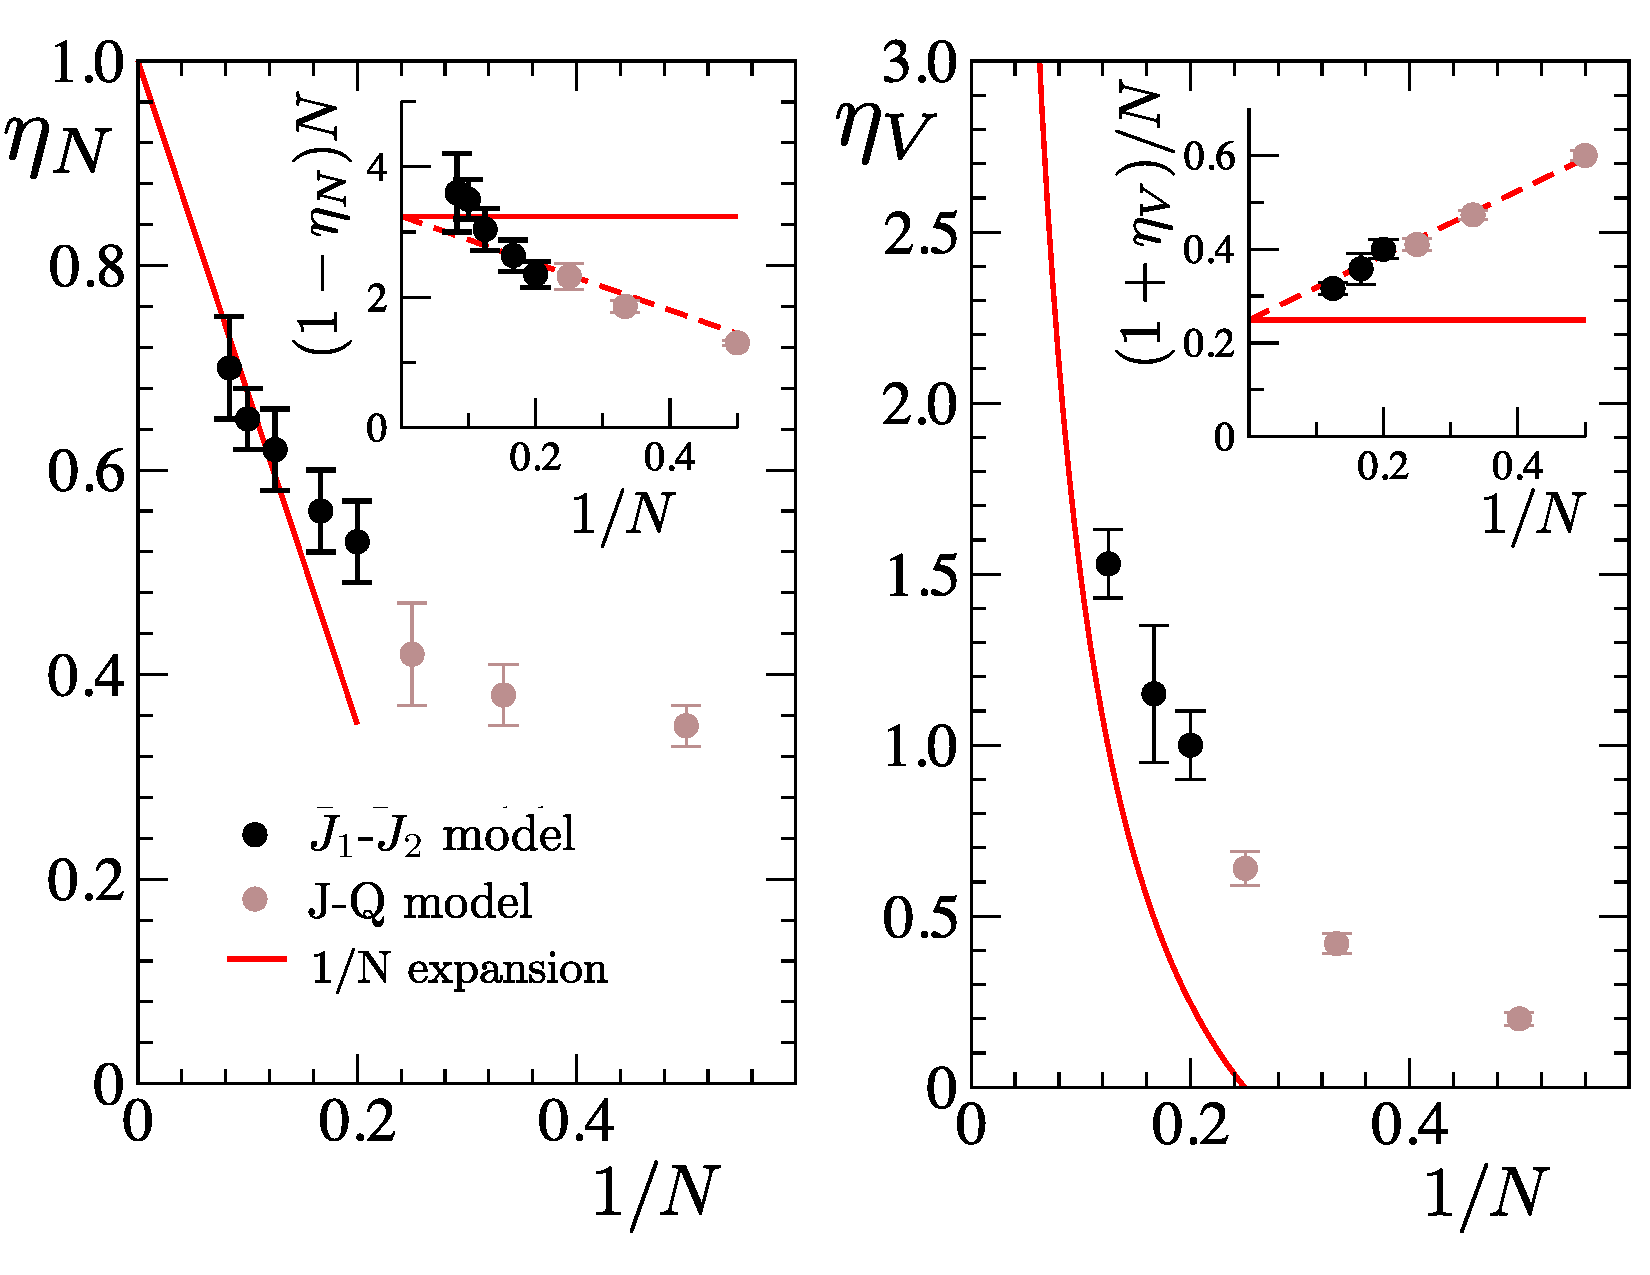
\includegraphics[width=3.0in]{fig_exp.pdf}
  \caption{ \label{fig:exp} Anomalous dimensions of the N\'eel (left)
    and VBS (right)
  order parameters as a function of $N$. The main panels show $\eta_N$ and $\eta_V$ versus $1/N$. For $N=2,3$ and $4$, the data are 
  for the J-Q model, and the results for $N>4$ are for the $J_1$-$J_2$ model. The analytic results 
  from the $1/N$ expansion of the CP$^{N-1}$ field theory are shown as thick red lines. The left and right insets 
  show $N(1-\eta_N)$ and $(1+\eta_V)/N$, respectively. These quantities must be finite in the  $N\rightarrow \infty$ 
  limit according to the DQC theory and should be given by Eq.~(\ref{eq:oneonN}) (solid straight lines in the insets). 
  The next corrections to the exponents have not been computed analytically yet, but we can estimate them approximately 
  as $1+\eta_V = 0.2492 N + 0.68(4)$, $\eta_N = 1+32/(\pi^2 N)-3.6(5)/N^2$ (shown as dashed lines).}
\end{figure}

\subsection{SU($N$) Bilayer}
\label{ss:bilN}

The bilayer geometry provides a simple way to force a trivial paramagnetic
state into the types of SU($N$) models we have discussed in this
section. Consider a bilayer in which each layer is described by some
combination of the $J_1$-$J_2$-$Q$ interactions. Now consider the
following coupling between the layers,
\begin{equation}
 H_{J_\perp} = -J_\perp \sum_{a,[ij]} T^a_i\cdot T^{*a}_j
\end{equation}
where the sum $[ij]$ is taken between spins vertically below each other
in the bilayer. The $J_\perp$ only model has a featureless non-degenerate ground state
consisting of a product of vertical valence bonds. The introduction of intra-layer couplings like the $J_1$-$J_2$-$Q$ interactions will
make the ground state deviate from a simple product state by
increasing the amount of entanglement, but these couplings
 cannot destabilize the featureless paramagnetic
state as long as they are small compared to $J_\perp$. 

{\em (show some data here? we need to decide which plots to show
  depending on the space)-- Ribhu}
\section{U(1) models}

As mentioned above, one of the main foci of research into designer Hamiltonians is the search, detection and characterization of quantum spin liquid (QSL) phases.  In the last few years, there have been several high-profile numerical studies identifying candidate spin liquid states in a variety of Hamiltonians.  As mentioned above, the apparent resolution of the long-standing question of the kagome-lattice antiferromagnet's QSL groundstate has come through large-scale DMRG calculations.  In what came as a surprise to many, quantum Monte Carlo simulations have purported to find a QSL phase in the half-filled Hubbard model on the honeycomb lattice.  This latter case, which has subsequently become the subject of intense theoretical study, highlights that the synergy between field theory and numerics is often driven by the latter.

models are difficult to connect directly to 
attempts to reconcile theory and experiment rely on phenomenological low-energy effective theories of QSLs.

The smoking gun signature for a spin liquid phase could be argued to be the identification of the emergent gauge symmetry

Contrary to some conjectures, the existence of the sign problem 

\begin{enumerate}
\item We have 4 or 5 Hamiltonians (with Z2 and U(1) spin liquids)
\item Balents Fisher Girvin gave us a ``recipe'' for creating Hamiltonians with Z2 spin liquids using constrained interactions
\item The connection to field theory is the emergent gauge structure I guess
\item Entanglement entropy identifies the emergent gauge structure of the underlying theory
\item XY*
\end{enumerate}

\section{Discussion}
- Many things left to do along these lines (give some examples), e.g., larger sizes are still needed
to fully characterize N\'eel--VBS transition; parallelization of QMC, impurities, disorder

- Fermions: it should be possible to study 1 or 2 fermions (manageble sign problem) in 
VBS/critical/spin-liquid systems. One should be able to see some aspects of the "strange metal''.
Mention meron algorithm---perhaps some more interesting designer hamiltonian can be constructed.

- Open fundamental questions in this approach, e.g., can one design a sign-problem-free
  SU(2) hamiltonian with a spin liquid phase?

- Non-equilibrium QMC

- Some blah-blah about the sign problem, e.g., mention, in some diplomatic way, that Troyer-Wiese ``proof'' of no 
solution is meaningless (classical glasses are also exponentially hard, so why should not quantum glasses be?---this
is all they ``prove''). Perhaps mention variational QMC in the context of tensor-network states.

% Create the reference section using BibTeX:
%\bibliography{}{}

\end{document}

